% Figure 2: 3x2 designer comparison — A5 vs. A6 grouped bar chart
% Snyder (Construction), Katz (Operational), Young (Perceptual)
% Scores /45; pass threshold = 33
% Self-contained figure environment — \input{} into main.tex.
% Requires: pgfplots, pgfplotsthemetol (or just pgfplots), tikz loaded in preamble.

\begin{figure}[htbp]
  \centering
  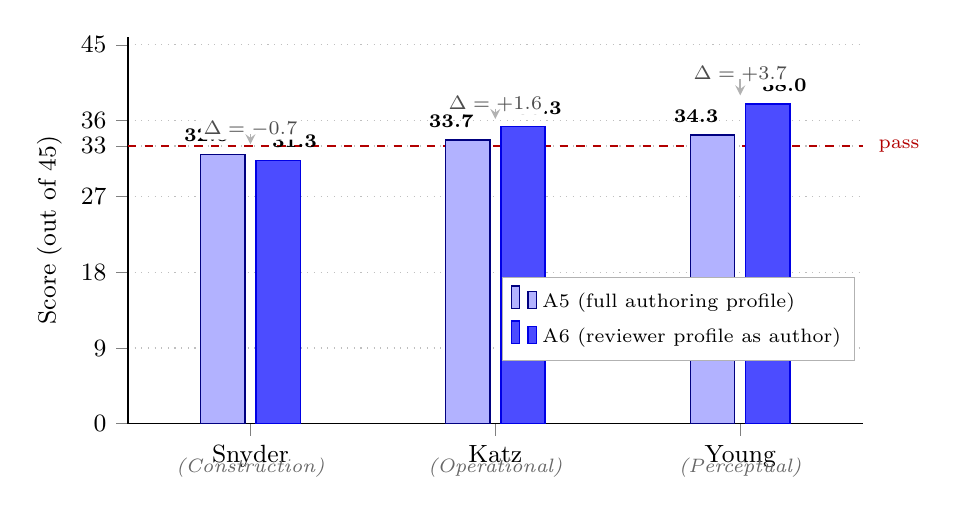
\begin{tikzpicture}
    \begin{axis}[
        ybar                  = 4pt,          % gap between bars in same group
        bar width             = 16pt,
        width                 = 0.90\columnwidth,
        height                = 6.5cm,
        enlarge x limits      = 0.25,
        ymin                  = 0,
        ymax                  = 46,
        ytick                 = {0,9,18,27,33,36,45},
        yticklabels           = {0,9,18,27,33,36,45},
        yticklabel style      = {font=\small},
        ylabel                = {Score (out of 45)},
        ylabel style          = {font=\small},
        xtick                 = {1,2,3},
        xticklabels           = {Snyder, Katz, Young},
        xticklabel style      = {font=\small},
        axis x line*          = bottom,
        axis y line*          = left,
        tick align            = outside,
        ymajorgrids           = true,
        grid style            = {dotted, gray!50},
        legend style          = {
            at                = {(0.99,0.38)},
            anchor            = north east,
            font              = \scriptsize,
            draw              = gray!60,
            fill              = white,
            cells             = {anchor=west},
            inner sep         = 3pt,
            row sep           = 1pt,
        },
        legend entries        = {%
            A5\ (full authoring profile),%
            A6\ (reviewer profile as author)%
        },
        clip                  = false,
    ]

    %% ---- pass threshold line at y=33 ----
    \draw[dashed, red!70!black, line width=0.8pt]
      (axis cs:0.5, 33) -- (axis cs:3.5, 33)
      node[pos=1.0, right, font=\scriptsize, text=red!70!black, xshift=2pt]
      {pass};

    %% ---- A5 bars (light blue) ----
    \addplot[
        fill      = blue!30,
        draw      = blue!50!black,
        line width = 0.5pt,
    ] coordinates {
        (1, 32.0)
        (2, 33.7)
        (3, 34.3)
    };

    %% ---- A6 bars (dark blue; Young bar hatched to mark dataset max) ----
    % Snyder and Katz A6
    \addplot[
        fill      = blue!70,
        draw      = blue!90!black,
        line width = 0.5pt,
    ] coordinates {
        (1, 31.3)
        (2, 35.3)
        (3, 38.0)
    };

    %% ---- score labels on bars ----
    %% A5 labels (left bar of each group: x offset ~-0.18)
    \node[above, font=\scriptsize\bfseries, yshift=1pt]
        at (axis cs:0.82, 32.0) {32.0};
    \node[above, font=\scriptsize\bfseries, yshift=1pt]
        at (axis cs:1.82, 33.7) {33.7};
    \node[above, font=\scriptsize\bfseries, yshift=1pt]
        at (axis cs:2.82, 34.3) {34.3};

    %% A6 labels (right bar of each group: x offset ~+0.18)
    \node[above, font=\scriptsize\bfseries, yshift=1pt]
        at (axis cs:1.18, 31.3) {31.3};
    \node[above, font=\scriptsize\bfseries, yshift=1pt]
        at (axis cs:2.18, 35.3) {35.3};
    \node[above, font=\scriptsize\bfseries, yshift=1pt]
        at (axis cs:3.18, 38.0) {38.0};

    %% ---- gap annotations above each bar pair ----
    % Snyder: gap = -0.7 (A6 < A5, slight decline)
    \node[font=\scriptsize, text=black!70,
          fill=white, inner sep=1pt, rounded corners=1pt]
        at (axis cs:1, 35.0) {$\Delta=-0.7$};
    \draw[-stealth, gray!60, line width=0.6pt]
        (axis cs:1, 34.4) -- (axis cs:1, 33.2);

    % Katz: gap = +1.6
    \node[font=\scriptsize, text=black!70,
          fill=white, inner sep=1pt, rounded corners=1pt]
        at (axis cs:2, 38.0) {$\Delta=+1.6$};
    \draw[-stealth, gray!60, line width=0.6pt]
        (axis cs:2, 37.4) -- (axis cs:2, 36.2);

    % Young: gap = +3.7
    \node[font=\scriptsize, text=black!70,
          fill=white, inner sep=1pt, rounded corners=1pt]
        at (axis cs:3, 41.5) {$\Delta=+3.7$};
    \draw[-stealth, gray!60, line width=0.6pt]
        (axis cs:3, 40.9) -- (axis cs:3, 39.0);

    %% ---- dataset-maximum star on Young A6 bar ----
    \node[font=\normalsize, text=orange!80!red]
        at (axis cs:3.18, 40.0) {$\bigstar$};

    %% ---- lens-type sub-labels below x-axis tick labels ----
    \node[font=\scriptsize\itshape, text=black!60, yshift=-16pt]
        at (axis cs:1, 0) {(Construction)};
    \node[font=\scriptsize\itshape, text=black!60, yshift=-16pt]
        at (axis cs:2, 0) {(Operational)};
    \node[font=\scriptsize\itshape, text=black!60, yshift=-16pt]
        at (axis cs:3, 0) {(Perceptual)};

    \end{axis}
  \end{tikzpicture}

  \caption{%
    Designer comparison: A5 (full authoring profile) vs.\ A6 (reviewer profile
    repurposed for authoring), for three designers. Gap is $\text{A6}-\text{A5}$.
    Katz's operational lens transfers positively; Snyder's construction lens shows
    near-zero gap; Young's perceptual lens produces the largest gap and the
    dataset-high score (38.0/45, marked~$\bigstar$) because the reviewer-as-author
    exercise forces a format-compatible substitution for her visual instincts.
  }
  \label{fig:designers}
\end{figure}
